\begin{figure}[t]
    \centering
    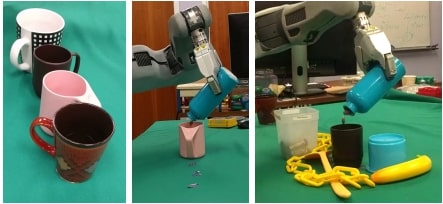
\includegraphics[width=0.6\textwidth]{figures/images/deep_object_centric_representation/pouring_task.jpg}
    \caption{Pouring task setting proposed in \cite{devin2018deep}. (Left) Mugs used for evaluation. Note that only the brown mug was seen during training. Center: Successful pouring into the pink mug. (Right) Pouring into the brown mug in a cluttered environment that was not seen during training.}
    \label{fig:pouring_task_setting}
\end{figure}

\begin{figure}[t]
    \centering
    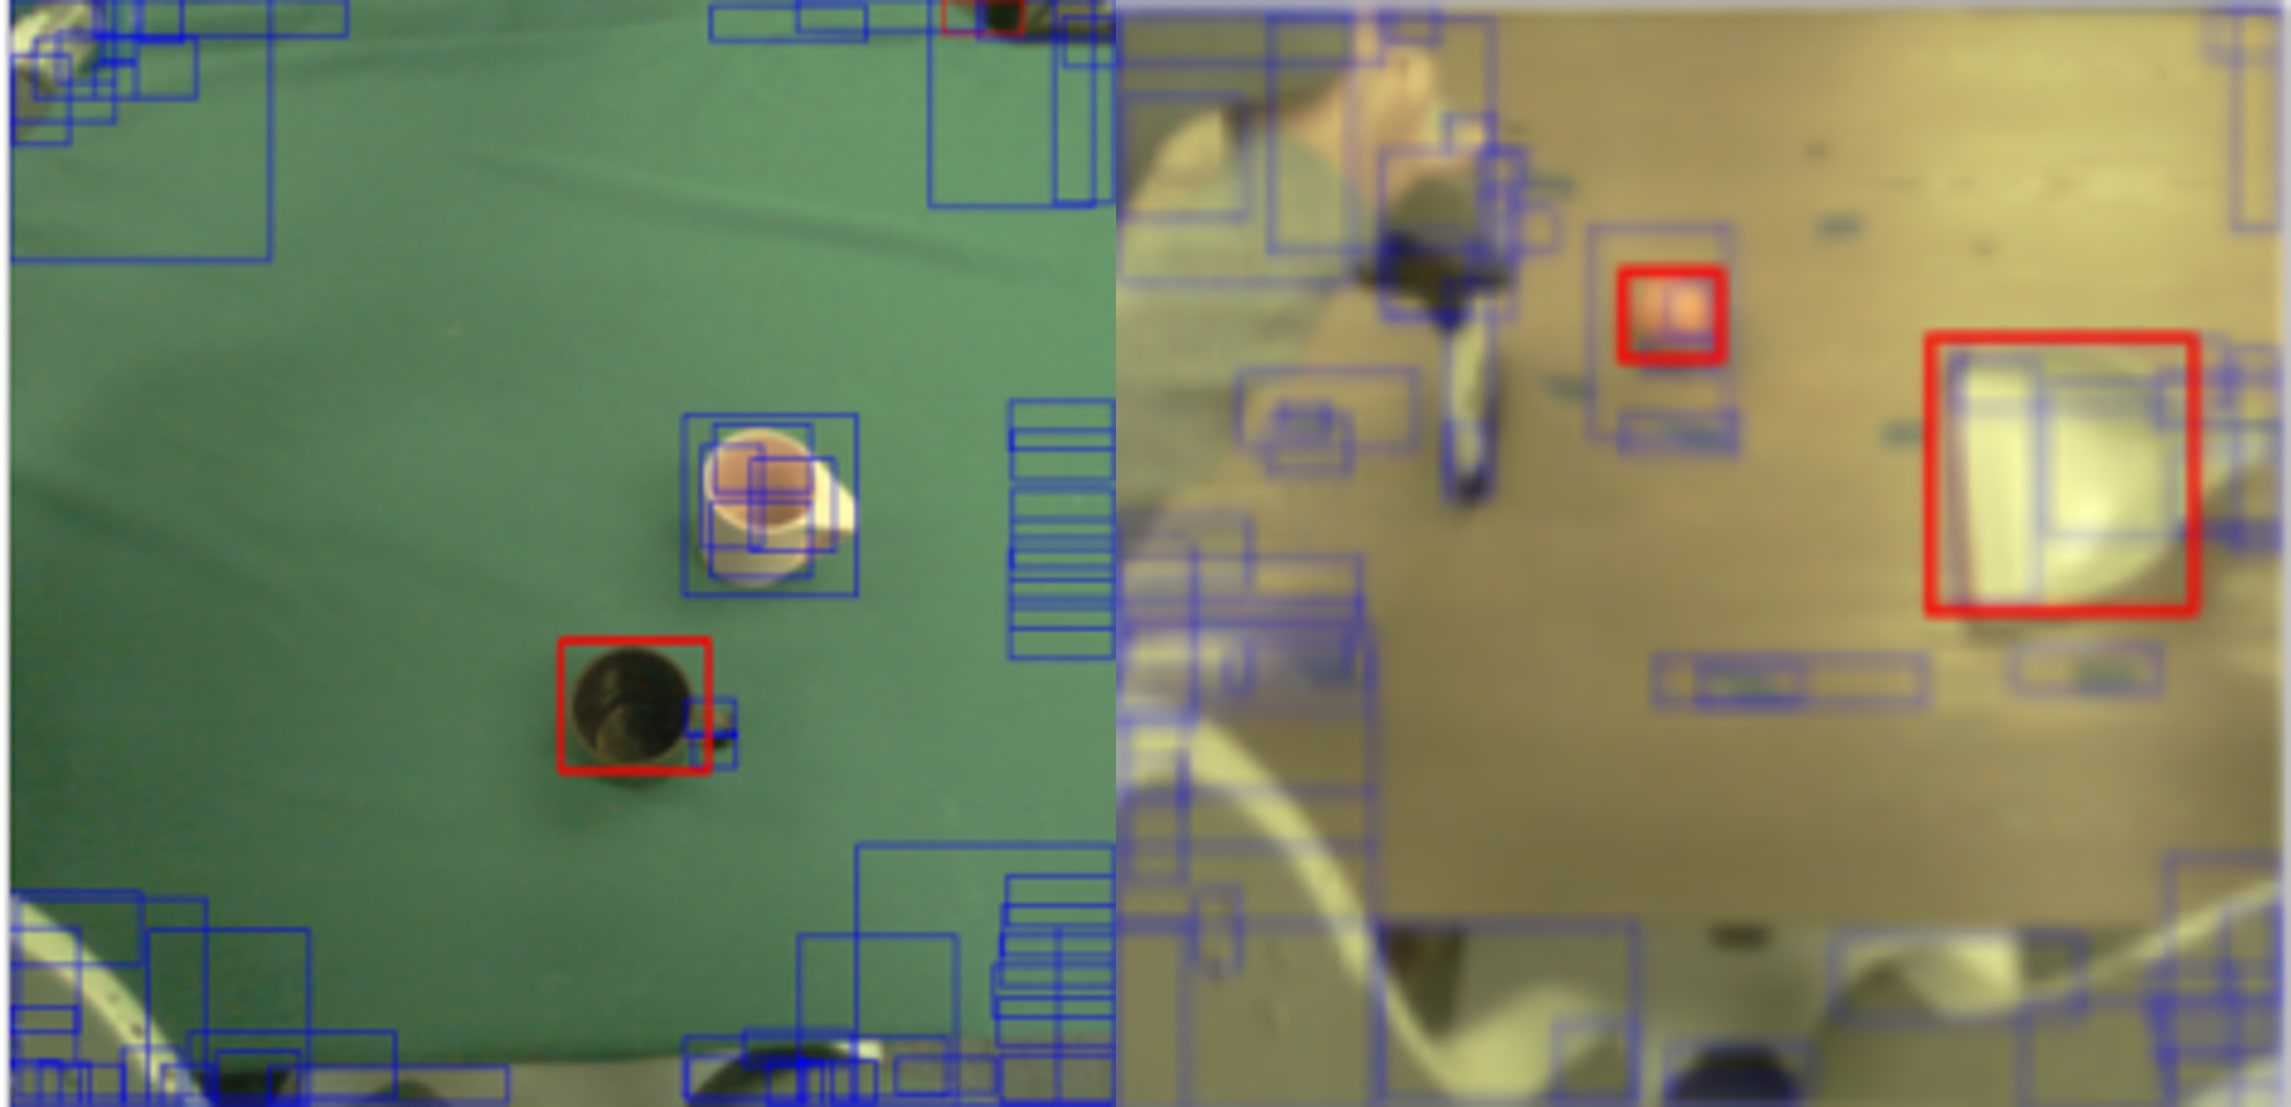
\includegraphics[width=0.6\textwidth]{figures/images/deep_object_centric_representation/mugs_distractors.jpg}
        \caption{The region proposals (meta-attention) are drawn in blue and the task-specific attended regions are drawn in red. For the Pouring task with distractor mug (pink) and target mug (brown), the attention locks on to the brown mug as its position defines the trajectory. For the sweeping task, two attention vectors are used, one attends to the orange and one attends to the dustpan.}
    \label{fig:task_specific_attention}
\end{figure}